\documentclass[dvipsnames,beamer,10pt]{standalone}

\usepackage{tikz}
\usetikzlibrary{positioning,decorations.pathreplacing,fit}
\usetikzlibrary{decorations.markings,arrows.meta,shapes.arrows,arrows}
\usetikzlibrary{calc}

\definecolor{mygreen}{RGB}{0,128,80}
\colorlet{darkgreen}{mygreen!90!black}


%\DeclareMathSizes{10.0}{12}{5}{4}


\begin{document}




\begin{standaloneframe}

\resizebox{0.8\textwidth}{!}{



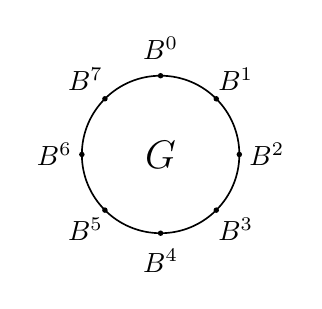
\begin{tikzpicture}[
	send/.style= {
		>={Latex[length=1pt,width=1.8pt]},shorten <= 1pt,line width=0.3pt
	},
	]
	
	\def\p{8}
	\pgfmathtruncatemacro{\pminus}{\p-1};
	\def\radius{1cm}
	
	\draw[semithick] circle(\radius) node {\Large $\mathbb{G}$};
	
	\foreach \a in {0,1,...,\pminus}{
		\draw (-\a*360/\p + 90: {\radius + 0.35cm}) node[xshift=0pt] (g\a) {$B^{\a}$};
		\draw (-\a*360/\p + 90: \radius) node [fill,circle, inner sep=0.7pt] {};
	}
	


\end{tikzpicture}


}

\end{standaloneframe}


\end{document}